%% LaTeX2e class for student theses
%%
%% Karlsruhe Institute of Technology
%% Institute of Information Security and Dependability
%% Software Design and Quality (SDQ)
%%
%% Dr.-Ing. Erik Burger
%% burger@kit.edu
%%
%% Version 1.6, 2024-06-07

\chapter{Implementation}
\label{ch:Implementation}

This chapter describes the implementation of the proposed \APE features to the \LiSSAf to optimize classification prompts.
As outlined in \autoref{ch:Approach}, the goal is to optimize prompts for a given set of \TLR tasks on a fixed dataset.
To achieve this goal, a new \promptoptimizer component is added to the \LiSSA pipeline.
This is elaborated in \autoref{sec:impl:prompt_optimizer_component}.
This component can be combined with further optional \metric and \evaluator components introduced in \autoref{sec:impl:metric_component} and \autoref{sec:impl:evaluator_component} to enable a flexible and reusable architecture.
The integration into the existing \LiSSA pipeline is explained in \autoref{sec:impl:lissa_integration}.

\begin{figure}
    \centering
    \includegraphics[width=\textwidth]{graphics/class_diagrams/components}
    \caption{Overview of the major new components involved in the implementation}
    \label{fig:component_diagramm}
\end{figure}

\autoref{fig:component_diagramm} provides an overview of the components involved in this implementation.
The \promptoptimizer component is the central part of the implementation.
The \method{optimize} method is used to optimize the prompt for a given set of \TLR tasks.
The source and target \elementstores as in the existing \LiSSA pipeline are provided as arguments to the method for training data.
The \metric component is used to score the quality of a prompt on a given set of tasks.
The \method{getMetric} method is used to retrieve the metric implementation for all prompts on set of classification tasks.
The \evaluator component is used to select a subset of tasks to evaluate the prompt on using the \metric.
Its \method{sampleAndEvaluate} method is used to selectively evaluate the prompts on a subset of tasks.
Ideally more evaluation budget is spent on prompts that are expected to perform better.


\section{Metric component}
\label{sec:impl:metric_component}
The \metric component provides implementations for different metrics to score the quality of a prompt on a given set of tasks.
Metrics can be divided into two major categories.
They are visualized in \autoref{fig:metric_component_diagramm}.
Pointwise metrics will evaluate each \TL prediction and return a separate score for each.
Scoring strategies for pointwise metrics are provided by the \scorer subcomponent.
The overall score can then be calculated by reducing the individual scores using a \reductor.
The \reductor subcomponent provides different strategies to reduce a collection of scores to a single value.
In contrast, global metrics will evaluate the entire set of \TL predictions at once and return a single score directly.
This is because they factor in relationships between different predictions, like whether the correct prediction is a true positive or a true negative.
The scores are cached using \LiSSAs built-in \cache component.

\begin{figure}
    \centering
    \fontsize{8}{10}\selectfont
    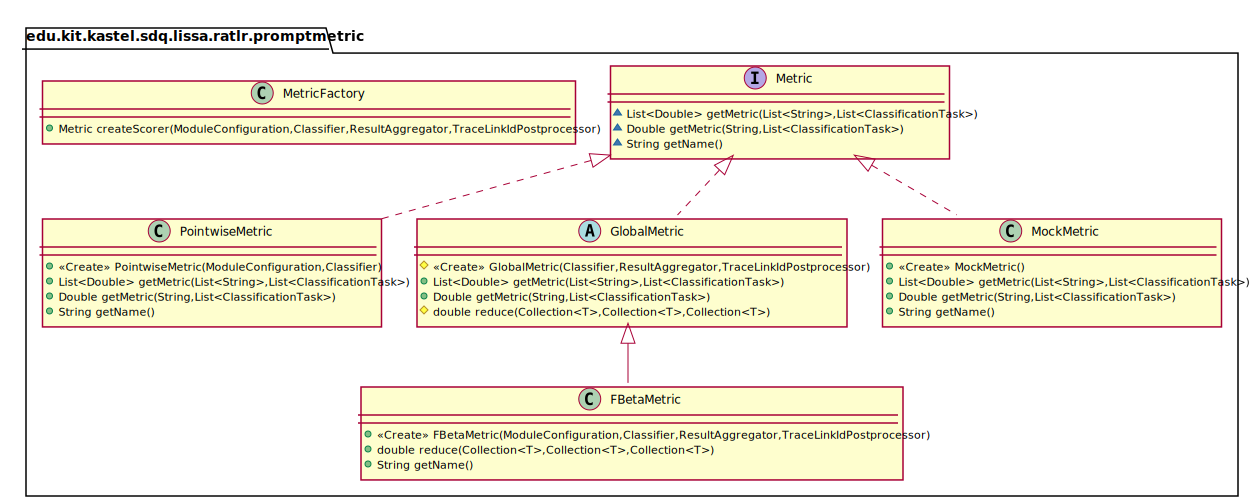
\includegraphics[width=\textwidth]{graphics/class_diagrams/metric}
    \caption{The new \metric component and its implementations}
    \label{fig:metric_component_diagramm}
\end{figure}

Currently, only the \fbeta metric is implemented as a global metric.
The beta parameter can be altered in the component configuration.
The score is computed utilizing a \method{reduce} method, that is provided the ground truth as well as the accepted and rejected values.

The pointwise metric implementation relies on the \method{Binary}\scorer and the \method{Mean}\reductor.
This is also portrayed in \autoref{fig:scorer_reductor_diagramm}.
A \scorer is required to implement the \method{score} logic for a list of tasks and their classified results.
The \method{Binary}\scorer will return a score of 1.0 for a correct prediction and 0.0 otherwise.
A correct prediction is defined as predicting a \TL for a pair of artifacts that actually has a \TL in the ground truth or not predicting a \TL for a pair of artifacts that does not have a \TL in the ground truth.
An \reductor is required to implement the \method{reduce} logic for a collection of individual scores.
The \method{Mean}\reductor will then compute the mean of all individual scores to return a single value.

\begin{figure}
    \centering
    \fontsize{8}{10}\selectfont
    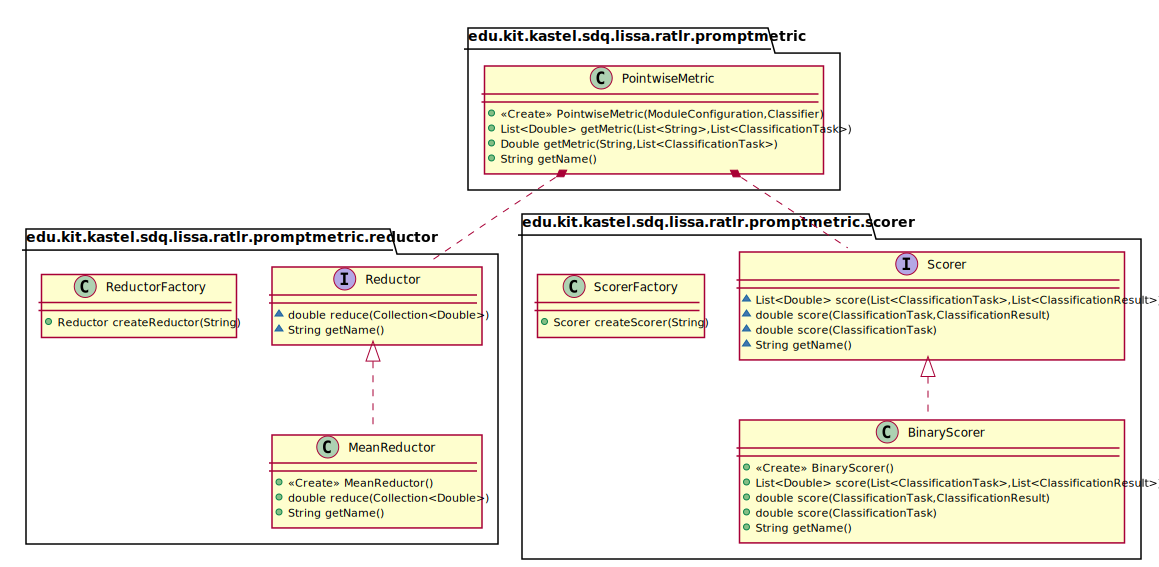
\includegraphics[width=\textwidth]{graphics/class_diagrams/pointwise_metric}
    \caption{The subcomponents utilized by the pointwise metric implementation}
    \label{fig:scorer_reductor_diagramm}
\end{figure}


\section{Evaluator component}
\label{sec:impl:evaluator_component}
The \evaluator component provides implementations to evaluate the quality of a prompt on a given set of tasks.
In contrast to the \metric component, the \evaluator will not use all tasks to compute the prompt score.
Instead, more complex sampling strategies can be used to select a subset of tasks.
This is especially useful for larger datasets, where evaluating all tasks would be too costly.
The \ucb bandit evaluator is the most noteworthy implementation.
It will use the \ucb algorithm to select a subset of tasks that are expected to provide the most information gain.
This is achieved by balancing exploration and exploitation.
The size of the subset can be configured in the component configuration.
The \ucb evaluator is supplied with a random seed to ensure reproducibility of results.


\section{Prompt Optimizer component}
\label{sec:impl:prompt_optimizer_component}

The prompt optimizer component provides implementations for the actual prompt optimization.
Concrete objects will be instantiated with a set of configuration parameters, again following the format of the \LiSSAf.
A factory class is used to create the object based on the configuration.
Furthermore, the \metric and \evaluator components are provided to the respective constructors if required.
The \metric component is used to score the quality of a prompt on a given set of tasks.
The \evaluator component is used to select a subset of tasks to evaluate the prompt on.
This component is designed to be used in the \LiSSA evaluation pipeline after the preprocessing of artifacts into \elementstore's is completed.
These steps are already part of the existing \LiSSA framework for evaluation.
They are explained in more detail in \autoref{sec:foundations:lissa}.
\newcommand{\optimizermethod}{\method{optimize}}
The only functionality required in the \promptoptimizer interface is the \optimizermethod method.
This method can also be seen in \autoref{fig:optimizer_component_diagramm}.
The \optimizermethod requires the source and target \elementstores created in the previous pipeline steps as arguments.
Using the retrieval strategy of the target \elementstore a set of candidate pairs of elements is created.
This set will also be referred to as the training data, on which the prompt will be optimized.

The prompt to be optimized is provided in the component configuration during the optimizers' instantiation.
The method will return the optimized prompt as a string.
When \promptoptimizer implementations utilize \classifiers, the training data or subsets will be passed on to the classification method, integrating into the existing \LiSSA classification pipeline.
Thus, utilizing \LiSSAs caching for the \LLM queries, the optimization is deterministic and reproducible.
All further implementations should also be deterministic and reproducible.
Configuration parameters such as random seed are used to ensure this.

\begin{figure}
    \centering
    \fontsize{8}{10}\selectfont
    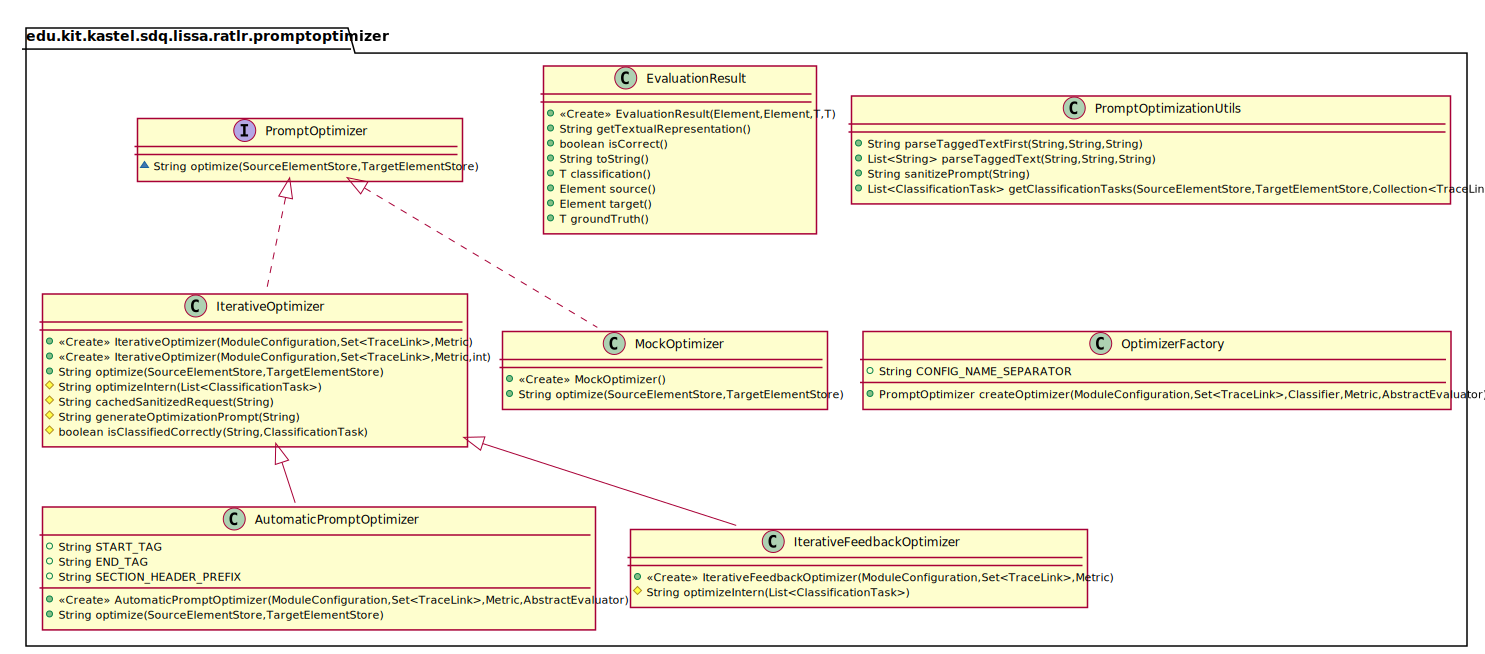
\includegraphics[width=\textwidth]{graphics/class_diagrams/optimizer}
    \caption{The new \promptoptimizer component and its implementations}
    \label{fig:optimizer_component_diagramm}
\end{figure}

The \promptoptimizer component will typically use the \LLM to evaluate different prompts.
Three different implementations are provided, as shown in \autoref{fig:optimizer_component_diagramm}.
The \method{optimizeIntern} is overwritten in the \method{IterativeFeedbackOptimizer} and to add the feedback of previously misclassified \TLs to the optimization prompt.
Combined with the \method{IterativeOptimizer} this implements the naive \APE algorithms from \autoref{approach:sec:naive_iterative}.
Many implementations of the \promptoptimizer component will require sampling strategies to reduce the number of calls to the \LLM.
This keeps the optimization cost manageable, as not every possible classification task is queried with the optimized prompt candidates.
This is achieved by introducing the new \samplingstrategy subcomponent.

The \samplingstrategy provides different strategies to select a sublist of comparable elements from a collection.
The strategies can be instantiated with configuration parameters and are used by the \promptoptimizer component.
This way, sampling strategies can be swapped easily without changing the actual optimization logic.
The random sampler uses a fixed random seed to ensure reproducibility of results.

\begin{figure}
    \centering
    \fontsize{8}{10}\selectfont
    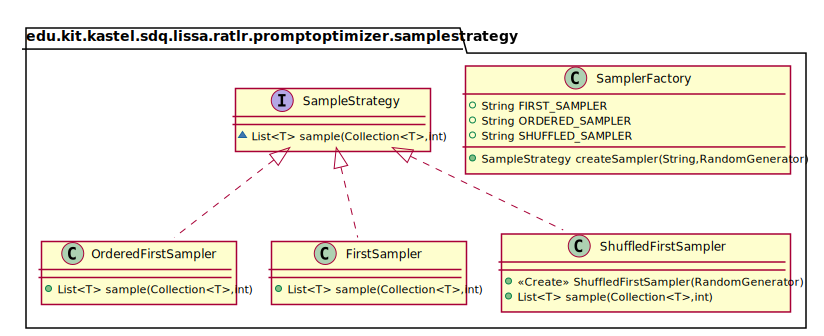
\includegraphics[width=\textwidth]{graphics/class_diagrams/sample_strategy}
    \caption{The new \samplingstrategy subcomponent and its implementations}
    \label{fig:sampling_strategy_diagramm}
\end{figure}

In \autoref{fig:sampling_strategy_diagramm}, the sampling strategy subcomponent is depicted.
The \method{sample} method is required to be implemented by all sampling strategies.
It will receive a collection of comparable elements and the desired sample size as arguments.
Currently, three different strategies are implemented.
\begin{itemize}
    \item The \method{ShuffledFirstSampler} will shuffle the input list using the \method{RandomGenerator} and return the first elements.
    \item The \method{OrderedFirstSampler} will sort the input list and return the first elements.
    \item The \method{FirstSampler} will return the first elements of the input list.
\end{itemize}


\section{LiSSA Pipeline Integration}
\label{sec:impl:lissa_integration}
The new components are integrated into the \LiSSA pipeline.
A new command was added to the \LiSSA command-line interface to run the prompt optimization.
The command will read the configuration file and create the required components using their constructors or factories, respectively.
To do so an evaluation pipeline object is created and relevant components will be retrieved from it.
This includes the classifier, aggregator, trace link id postprocessor as well as the source and target \elementstore's.
The classifier component is used to classify a pair of elements having a \TL or not during the optimization process.

The features integrate seamlessly into the existing \LiSSA architecture, espcially existing evaluation configurations can still be used.
The current classifiers can be utilized by the \metric implementations to classify pairs of elements during the optimization process.
This enables optimization of both zero-shot and chain-of-thought classification prompts.
The \ToT classification utilizes the existing \classifiers in \LiSSA as well.
To integrate sampling of optimization candidates, the \classifiers are extended to modify their classification prompt.
This functionality is only used by the \metric component.

While the optimization pipeline, as a standalone, is independent of the regular evaluation pipeline, they can be combined.
This is achieved by feeding the optimized prompt from the optimization pipeline into the evaluation pipeline, indicated by a separate configuration.
End-to-end tests are provided to ensure the correct integration of the new features into the existing \LiSSA framework.
The implementation is open source and available in the \replicationPackage.
